% Options for packages loaded elsewhere
% Options for packages loaded elsewhere
\PassOptionsToPackage{unicode}{hyperref}
\PassOptionsToPackage{hyphens}{url}
\PassOptionsToPackage{dvipsnames,svgnames,x11names}{xcolor}
%
\documentclass[
  10pt,
  letterpaper,
  DIV=11,
  numbers=noendperiod]{scrartcl}
\usepackage{xcolor}
\usepackage{amsmath,amssymb}
\setcounter{secnumdepth}{5}
\usepackage{iftex}
\ifPDFTeX
  \usepackage[T1]{fontenc}
  \usepackage[utf8]{inputenc}
  \usepackage{textcomp} % provide euro and other symbols
\else % if luatex or xetex
  \usepackage{unicode-math} % this also loads fontspec
  \defaultfontfeatures{Scale=MatchLowercase}
  \defaultfontfeatures[\rmfamily]{Ligatures=TeX,Scale=1}
\fi
\usepackage{lmodern}
\ifPDFTeX\else
  % xetex/luatex font selection
\fi
% Use upquote if available, for straight quotes in verbatim environments
\IfFileExists{upquote.sty}{\usepackage{upquote}}{}
\IfFileExists{microtype.sty}{% use microtype if available
  \usepackage[]{microtype}
  \UseMicrotypeSet[protrusion]{basicmath} % disable protrusion for tt fonts
}{}
% Make \paragraph and \subparagraph free-standing
\makeatletter
\ifx\paragraph\undefined\else
  \let\oldparagraph\paragraph
  \renewcommand{\paragraph}{
    \@ifstar
      \xxxParagraphStar
      \xxxParagraphNoStar
  }
  \newcommand{\xxxParagraphStar}[1]{\oldparagraph*{#1}\mbox{}}
  \newcommand{\xxxParagraphNoStar}[1]{\oldparagraph{#1}\mbox{}}
\fi
\ifx\subparagraph\undefined\else
  \let\oldsubparagraph\subparagraph
  \renewcommand{\subparagraph}{
    \@ifstar
      \xxxSubParagraphStar
      \xxxSubParagraphNoStar
  }
  \newcommand{\xxxSubParagraphStar}[1]{\oldsubparagraph*{#1}\mbox{}}
  \newcommand{\xxxSubParagraphNoStar}[1]{\oldsubparagraph{#1}\mbox{}}
\fi
\makeatother


\usepackage{longtable,booktabs,array}
\usepackage{calc} % for calculating minipage widths
% Correct order of tables after \paragraph or \subparagraph
\usepackage{etoolbox}
\makeatletter
\patchcmd\longtable{\par}{\if@noskipsec\mbox{}\fi\par}{}{}
\makeatother
% Allow footnotes in longtable head/foot
\IfFileExists{footnotehyper.sty}{\usepackage{footnotehyper}}{\usepackage{footnote}}
\makesavenoteenv{longtable}
\usepackage{graphicx}
\makeatletter
\newsavebox\pandoc@box
\newcommand*\pandocbounded[1]{% scales image to fit in text height/width
  \sbox\pandoc@box{#1}%
  \Gscale@div\@tempa{\textheight}{\dimexpr\ht\pandoc@box+\dp\pandoc@box\relax}%
  \Gscale@div\@tempb{\linewidth}{\wd\pandoc@box}%
  \ifdim\@tempb\p@<\@tempa\p@\let\@tempa\@tempb\fi% select the smaller of both
  \ifdim\@tempa\p@<\p@\scalebox{\@tempa}{\usebox\pandoc@box}%
  \else\usebox{\pandoc@box}%
  \fi%
}
% Set default figure placement to htbp
\def\fps@figure{htbp}
\makeatother





\setlength{\emergencystretch}{3em} % prevent overfull lines

\providecommand{\tightlist}{%
  \setlength{\itemsep}{0pt}\setlength{\parskip}{0pt}}



 


\usepackage{xcolor, soul}
\definecolor{Light}{gray}{.90}
\sethlcolor{Light}
\let\OldTexttt\texttt
\renewcommand{\texttt}[1]{\OldTexttt{\hl{#1}}}
\usepackage{caption}
\captionsetup{font=small, labelfont=bf}
\setlength{\parindent}{0pt}
\setlength{\parskip}{1.25ex}
% Symbols %%%%%%%%%%%%%%%%%%%%%%%%%%%%%%%%%%%%%%%%%%%%%%%%%%%%%

\usepackage{amsthm}
\usepackage{amsmath}
\usepackage{amssymb}
\usepackage{amsfonts}

% New commands %%%%%%%%%%%%%%%%%%%%%%%%%%%%%%%%%%%%%%%%%%%%%%%%

% General mathematical symbols
% argmin help from egreg from tex.stackexchange.com/questions/5223
\newcommand{\R}{\mathbb{R}}
\newcommand{\onedim}{\mathbb{R}}
\newcommand{\ddim}{\mathbb{R}^d}
\newcommand{\kdim}{\mathbb{R}^k}

\newcommand{\eps}{\varepsilon}
\newcommand{\seq}[1]{\{ #1_{n} \}}

\DeclareMathOperator*{\sign}{sign}
\DeclareMathOperator*{\argmin}{arg\,min}
\DeclareMathOperator*{\argmax}{arg\,max}

% boldface
\newcommand{\bfH}{\mathbf{H}}
\newcommand{\bfI}{\mathbf{I}}
\newcommand{\bfO}{\mathbf{O}}
\newcommand{\bfU}{\mathbf{U}}
\newcommand{\bfu}{\mathbf{u}}
\newcommand{\bfV}{\mathbf{V}}
\newcommand{\bfv}{\mathbf{v}}
\newcommand{\bfW}{\mathbf{W}}
\newcommand{\bfw}{\mathbf{w}}
\newcommand{\bfG}{\mathbf{G}}
\newcommand{\bfX}{\mathbf{X}}
\newcommand{\bfx}{\mathbf{x}}
\newcommand{\bfY}{\mathbf{Y}}
\newcommand{\bfy}{\mathbf{y}}
\newcommand{\bfZ}{\mathbf{Z}}
\newcommand{\bfz}{\mathbf{z}}
\newcommand{\bfmu}{\boldsymbol{\mu}}
\newcommand{\bfeps}{\boldsymbol{\epsilon}}
\newcommand{\bfbeta}{\boldsymbol{\beta}}
\newcommand{\bfgamma}{\boldsymbol{\gamma}}
\newcommand{\bfS}{\mathbf{S}}
\newcommand{\bfB}{\mathbf{B}}

% Sets
\newcommand{\setA}{\mathcal{A}}
\newcommand{\setB}{\mathcal{B}}
\newcommand{\setC}{\mathcal{C}}
\newcommand{\setF}{\mathcal{F}}
\newcommand{\rademacher}{\mathcal{R}}
\newcommand{\setP}{\mathcal{P}}

% General stats
\newcommand{\E}{\mathbb{E}}
\DeclareMathOperator*{\var}{Var}
\DeclareMathOperator*{\cor}{Corr}
\DeclareMathOperator*{\cov}{Cov}
\newcommand{\prob}{\mathbb{P}}

\newcommand{\indep}{\perp \!\!\! \perp}
\newcommand{\depen}{\cancel{\indep}}
\newcommand{\indic}{\mathbbm{1}}
\newcommand{\Xbar}{\overline{X}_n}
\newcommand{\Xsqbar}{\overline{X^2_n}}
\newcommand{\Xbarsq}{\overline{X}^2_n}
\newcommand{\Ybar}{\overline{Y}_n}
\newcommand{\lik}{\mathcal{L}}
\newcommand{\ton}[1]{#1_1, \dots, #1_n}
\newcommand{\fisher}{\mathcal{I}}
\newcommand{\sumn}{\sum_{i = 1}^n}
\newcommand{\prodn}{\prod_{i = 1}^n}

% Distributions
\newcommand{\hpp}{\textrm{HPP}}
\newcommand{\ipp}{\textrm{IPP}}
\newcommand{\geom}{\textrm{Geom}}
\newcommand{\iid}{\overset{\textrm{i.i.d.}}{\sim}}
\newcommand{\pois}{\textrm{Pois}}
\newcommand{\bern}{\textrm{Bern}}
\newcommand{\N}{\mathcal{N}}
\newcommand{\MVN}{\textrm{MVN}}
\newcommand{\unif}{\textrm{Unif}}
\newcommand{\binomial}{\textrm{Binom}}
\newcommand{\expo}{\textrm{Expo}}
\newcommand{\hgeom}{\textrm{HGeom}}

\KOMAoption{captions}{tableheading}
\makeatletter
\@ifpackageloaded{caption}{}{\usepackage{caption}}
\AtBeginDocument{%
\ifdefined\contentsname
  \renewcommand*\contentsname{Table of contents}
\else
  \newcommand\contentsname{Table of contents}
\fi
\ifdefined\listfigurename
  \renewcommand*\listfigurename{List of Figures}
\else
  \newcommand\listfigurename{List of Figures}
\fi
\ifdefined\listtablename
  \renewcommand*\listtablename{List of Tables}
\else
  \newcommand\listtablename{List of Tables}
\fi
\ifdefined\figurename
  \renewcommand*\figurename{Figure}
\else
  \newcommand\figurename{Figure}
\fi
\ifdefined\tablename
  \renewcommand*\tablename{Table}
\else
  \newcommand\tablename{Table}
\fi
}
\@ifpackageloaded{float}{}{\usepackage{float}}
\floatstyle{ruled}
\@ifundefined{c@chapter}{\newfloat{codelisting}{h}{lop}}{\newfloat{codelisting}{h}{lop}[chapter]}
\floatname{codelisting}{Listing}
\newcommand*\listoflistings{\listof{codelisting}{List of Listings}}
\makeatother
\makeatletter
\makeatother
\makeatletter
\@ifpackageloaded{caption}{}{\usepackage{caption}}
\@ifpackageloaded{subcaption}{}{\usepackage{subcaption}}
\makeatother
\usepackage{bookmark}
\IfFileExists{xurl.sty}{\usepackage{xurl}}{} % add URL line breaks if available
\urlstyle{same}
\hypersetup{
  pdftitle={Split-half correlations on earlier or shorter windows},
  pdfauthor={Al Xin},
  colorlinks=true,
  linkcolor={blue},
  filecolor={Maroon},
  citecolor={Blue},
  urlcolor={Blue},
  pdfcreator={LaTeX via pandoc}}


\title{Split-half correlations on earlier or shorter windows}
\author{Al Xin}
\date{Sep 17, 2026}
\begin{document}
\maketitle


\section{Takeaways}\label{takeaways}

\begin{itemize}
\tightlist
\item
  Split-half correlations for earlier and shorter windows align with the
  original split-half correlations.
\item
  IT is an exception, since earlier and shorter windows produce very low
  split-half correlations.
\item
  The between-family trend stays similar, though IT distances are lower
  relative to V4 (likely due to the difficulty in matching
  correlations). The trend also appears in noisy textures.
\item
  The between-sample trend changes, with V1 trending higher, possibly
  higher than V4 and IT. V2 remains the ``best''.
\item
  The changes require more investigation, as the correlations are harder
  to match with the new averages. The results may be confounded with the
  distribution of the reliabilities.
\end{itemize}

\section{Split-half correlations with other onset time
schemes}\label{split-half-correlations-with-other-onset-time-schemes}

Here, I check if the previous between-family and between-sample results
are consistent if the onsets are shifted earlier or if the averaging
window is shorter.

The calculations for the new split-half correlations can be found in
\texttt{scripts/split\_corrs\_earlier\_onsets.R} and associated bash
script.

\subsection{Comparison of original onsets and earlier onsets over
shorter
windows}\label{comparison-of-original-onsets-and-earlier-onsets-over-shorter-windows}

To capture initial firing, I calculated split-half correlations over
earlier onset times with shorter windows (100 ms vs.~the original 150
ms). These earlier, shorter split-half correlations are fairly well
correlated with the original split-half correlations
(Figure~\ref{fig-split_corrs_vs}). However, in IT, the earlier, shorter
correlations tend to be closer to zero, which is not surprising
considering 60 to 160 ms barely captures the averaged response curve
(not shown).

The distributions of the correlations for each condition can be seen in
Figure~\ref{fig-split_corrs_vs_hist}. For V1, taking earlier and shorter
windows appears to slightly increase the split-half correlations. This
trend reverses for the other regions.

\begin{figure}

\centering{

\pandocbounded{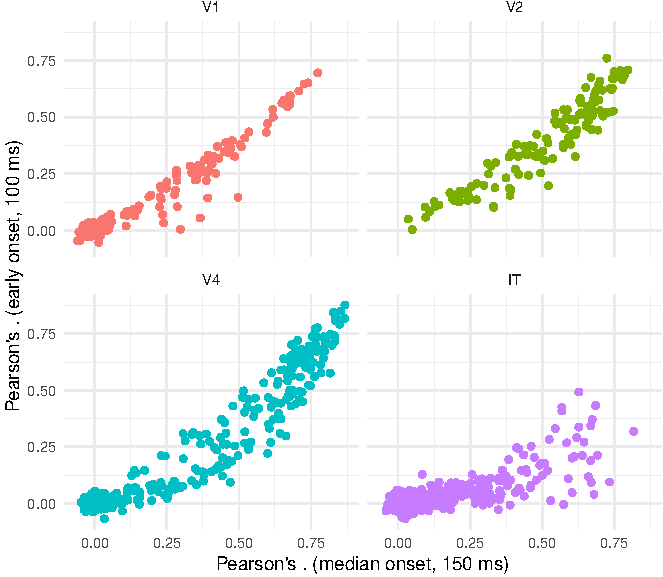
\includegraphics[keepaspectratio]{20260917_files/figure-pdf/fig-split_corrs_vs-1.pdf}}

}

\caption{\label{fig-split_corrs_vs}Scatter plots comparing the per-site
split-half correlations when onset times are earlier with 100 ms window
vs.~median with 150 ms window.}

\end{figure}%

\begin{figure}

\centering{

\pandocbounded{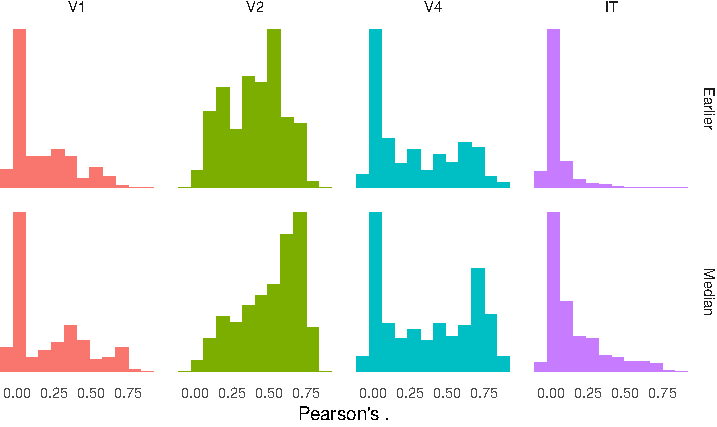
\includegraphics[keepaspectratio]{20260917_files/figure-pdf/fig-split_corrs_vs_hist-1.pdf}}

}

\caption{\label{fig-split_corrs_vs_hist}Histograms comparing the
per-site split-half correlations when onset times are earlier with 100
ms window vs.~median with 150 ms window.}

\end{figure}%

\section{Between-family distances}\label{between-family-distances}

The IT reliabilities are pretty low, so it's not easy to get
matched-reliability results with the previous method (selecting sites
with correlations in some interval). In Figure~\ref{fig-family}, IT dips
below V4, likely as a result of the low reliabilities. Otherwise, V1
\textless{} V2 \textless{} V4, as expected.

Unlike the previous results, the trend also emerges in noisy images.

\begin{figure}

\centering{

\pandocbounded{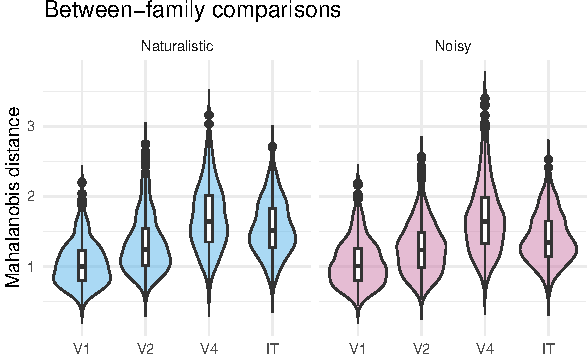
\includegraphics[keepaspectratio]{20260917_files/figure-pdf/fig-family-1.pdf}}

}

\caption{\label{fig-family}Mahalanobis distances in pairwise family
comparisons with earlier, shorter windows.}

\end{figure}%

\section{Between-sample distances}\label{between-sample-distances}

Unlike the previous results, the V1 results seem to be better than V4
and IT. V2 remains the ``best'' (Figure~\ref{fig-sample}).

\section{Between-sample comparisons}\label{between-sample-comparisons}

\begin{figure}

\centering{

\pandocbounded{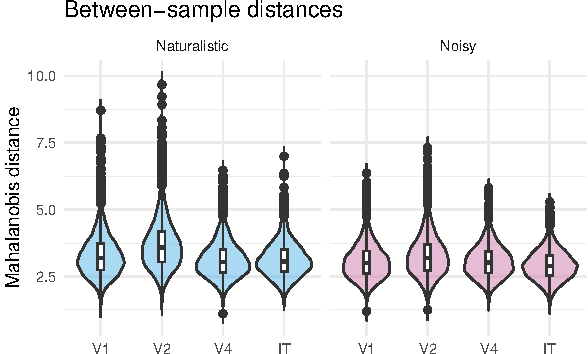
\includegraphics[keepaspectratio]{20260917_files/figure-pdf/fig-sample-1.pdf}}

}

\caption{\label{fig-sample}Mahalanobis distances in pairwise sample
comparisons with earlier, shorter windows.}

\end{figure}%

\section{References}\label{references}

\phantomsection\label{refs}




\end{document}
